%-----------------------------------------------------------------------------%
\chapter{\babDua}
%-----------------------------------------------------------------------------%

%-----------------------------------------------------------------------------%
\section{Kajian Penelitian Terkait}
%-----------------------------------------------------------------------------%
Banyak sekali referensi yang menjadi bagian besar dalam tertulisnya proposal ini, referensi tersebut terdiri atas berbagai macam jenis literatur dari sumber yang dapat diakses secara daring. Tak sedikit pula literatur tersebut menjadi alasan besar latar belakang dari proposal ini dilahirkan, berikut adalah beberapa penelitian terdahulu yang menjadi referensi dalam melakukan penyusunan proposal ini :
% Penelitian Terdahulu
\begin{center}
	\newcolumntype{L}[1]{>{\raggedright\let\newline\\\arraybackslash\hspace{1pt}}m{#1}}
	\newcolumntype{C}[1]{>{\centering\let\newline\\\arraybackslash\hspace{1pt}}m{#1}}
	\newcolumntype{R}[1]{>{\raggedleft\let\newline\\\arraybackslash\hspace{1pt}}m{#1}}
	
	\begin{longtable}{|>{\centering\arraybackslash}p{0.6cm}|p{4cm}|p{3cm}|p{5cm}|}
	\caption{Penelitian Terdahulu}
	\label{tab:table1}\\
	
	\hline
	\textbf{No.} & \textbf{Judul} & \textbf{Penulis} & \textbf{Hasil}\\
	\hline
	
	1.& \textit{Real Time Implementation of FMCW Radar for Target Detection Using GNURadio and USRP} \cite{Sundaresan2015}
	& Sundaresan S; Anjana C; Zacharia, Tessy; Gandhiraj R 	
	& Penggunaan radar FMCW dengan GNURadio lewat USRP N210 dan antena \textit{Log-periodic} bekerja dengan baik pada frekuensi 1GHz.\\ \hline
	
	2. & \textit{FMCW Radar Implemented with GNURadio Companion} \cite{Zhu2016}
	& Qizhao Zhu; Yaqi Wang 
	& Penggunaan GNURadio untuk simulasi radar FMCW sangat baik karena tanpa biaya dan memiliki tingkat kompleksitas yang rendah\\ \hline
	
	3. & \textit{Stationary and moving targets detection on FMCW radar using GNU radio-based software defined radio}\cite{Aulia2015}
	& Aulia, Siska; Suksmono, Andriyan Bayu; Munir, Achmad
	& Implementasi radar FMCW dengan GNURadio dan diolah di Matlab berhasil menunjukkan kemampuan radar dalam mendeteksi jarak target, melakukan kalkulasi tentang kecepatan relatif, dan memprediksi arah gerak target terhadap radar.\\ \hline
	
	4. & Implementasi Sistem Radar Frequency Modulated Continuous Wave Untuk Deteksi Jarak Berbasis USRP\cite{Saputro2019}
	& Saputro, Achmad Cahyo; Arseno, Dharu; Pramudita, A. A.
	& Implementasi radar FMCW dengan GNURadio lewat USRP N210 dengan bandwidth 10 MHz dan frekuensi 1 GHz bekerja dengan baik. \\ \hline
	
	5. & \textit{Implementation of a GNU radio and python FMCW radar toolkit }\cite{Mathumo2017}
	& Mathumo, Themba W.; Swart, Theo G.; Focke, Richard W.
	& Implementasi radar FMCW dengan GNUradio lewat USRP B210 dapat bekerja hingga jarak 150 m. Radar bekerja pada \textit{center frequency} 5.5 GHz dengan \textit{bandwidth} 28 MHz resolusi yang dicapai sekitar 5.35 m. \\ \hline
	
	6. & \textit{Linear Frequency Modulated Continous Wave Radar Using GNU Radio and USRP}  \cite{Saputera2015}
	& Saputera, Yussi Perdana; Herdiana, Dina; Madinawati, Hanny; Andriyan Bayu Suksmono, Achmad Munir
	& Penggunaan radar Linear FMCW yang diimplementasikan dengan GNURadio dan USRP bekerja dengan baik dan dapat mendeteksi hingga 3 objek pada jarak yang berbeda. \\ \hline
	
	7. & \textit{Accuracy analysis of FM chirp in GNU radio-based FMCW radar for multiple target detection} \cite{Amin2014}
	& Amin, Ershad Junus; Suksmono, Andriyan Bayu; Munir, Achmad
	& Penggunaan FM chirp pada radar FMCW yang diimplementasikan dengan GNURadio dianalisa. Dilakukan perbandingan antara 3 jenis gelombang, dengan frekuensi 1.5 MHz dan \textit{sample rate} 6Msps. Ditemukan bahwa akurasi tertinggi ada pada gelombang segitiga. \\ \hline
	
	8. & \textit{FMCW radar implemented in SDR architecture using a USRP device}\cite{Stasiak2017}
	& Stasiak, Krzysztof; Samczynski, Piotr
	& Implementasi FMCW radar dengan USRP telah dilakukan menggunakan frekuensi carrier 5.8 GHz. Ditemukan bahwa implementasi bekerja dengan baik, namun perlu dilakukannya riset agar dapat melakukan deteksi real time. \\ \hline
	
	9. & \textit{GNU Radio based software-defined FMCW radar for weather surveillance application}\cite{Prabaswara2011}
	& Prabaswara, Aditya; Munir, Achmad; Suksmono, Andriyan Bayu
	& Penggunaan FMCW radar dengan GNU radio lewat USRP N210 telah diimplementasikan untuk mengawasi cuaca. Radar bekerja pada frekuensi 2.1 GHz dengan bandwidth 750 kHz. Hasil menemukan bahwa prototipe dapat melakukan pengukuran jarak, maka diasumsikan bahwa prototipe dapat melakukan pendeteksi Gerakan partikel, posisi, dan intensitas. \\ \hline
	\end{longtable}
\end{center}
%-----------------------------------------------------------------------------%
%\section{Teori Dasar}
%-----------------------------------------------------------------------------%
\section{\textit{Software Defined Radio}}
\textit{Software Defined Radio} atau yang sering disingkat menjadi SDR merupakan teknologi komunikasi berbasis nirkabel yang kegunaannya dapat ditentukan oleh perangkat lunak \cite{Anisah2018}. Sehingga dalam implementasinya, tidak perlu dilakukan perubahan perangkat keras baru bila ingin melakukan perubahan, baik dari segi standar, teknologi, dan layanan. Hanya dengan melakukan perubahan konfigurasi saja, lalu SDR akan langsung dapat digunakan. 

Dalam implementasinya, SDR membutuhkan \textit{Universal Software Radio Peripheral}, atau yang sering disingkat menjadi USRP merupakan \textit{hardware} yang merupakan bagian \textit{front end} pada arsitektur sistem SDR. USRP terdiri dari modul yang dapat terkoneksi dengan komputer sehingga memperbolehkan pemrograman dengan aplikasi seperti GNURadio dan LabVIEW \cite{Gulo2023}. 

Penggunaan USRP sangat memudahkan proses perancangan prototipe dan pengujian karena adanya antarmuka yang dapat mengkoneksikan USRP dengan antena dan berbagai macam bagian perangkat keras yang dibutuhkan.

\subsection{\textit{Universal Software Radio Peripheral}}
\begin{center}
	\begin{figure}[h!]
		\begin{subfigure}[b]{0.5\linewidth}
			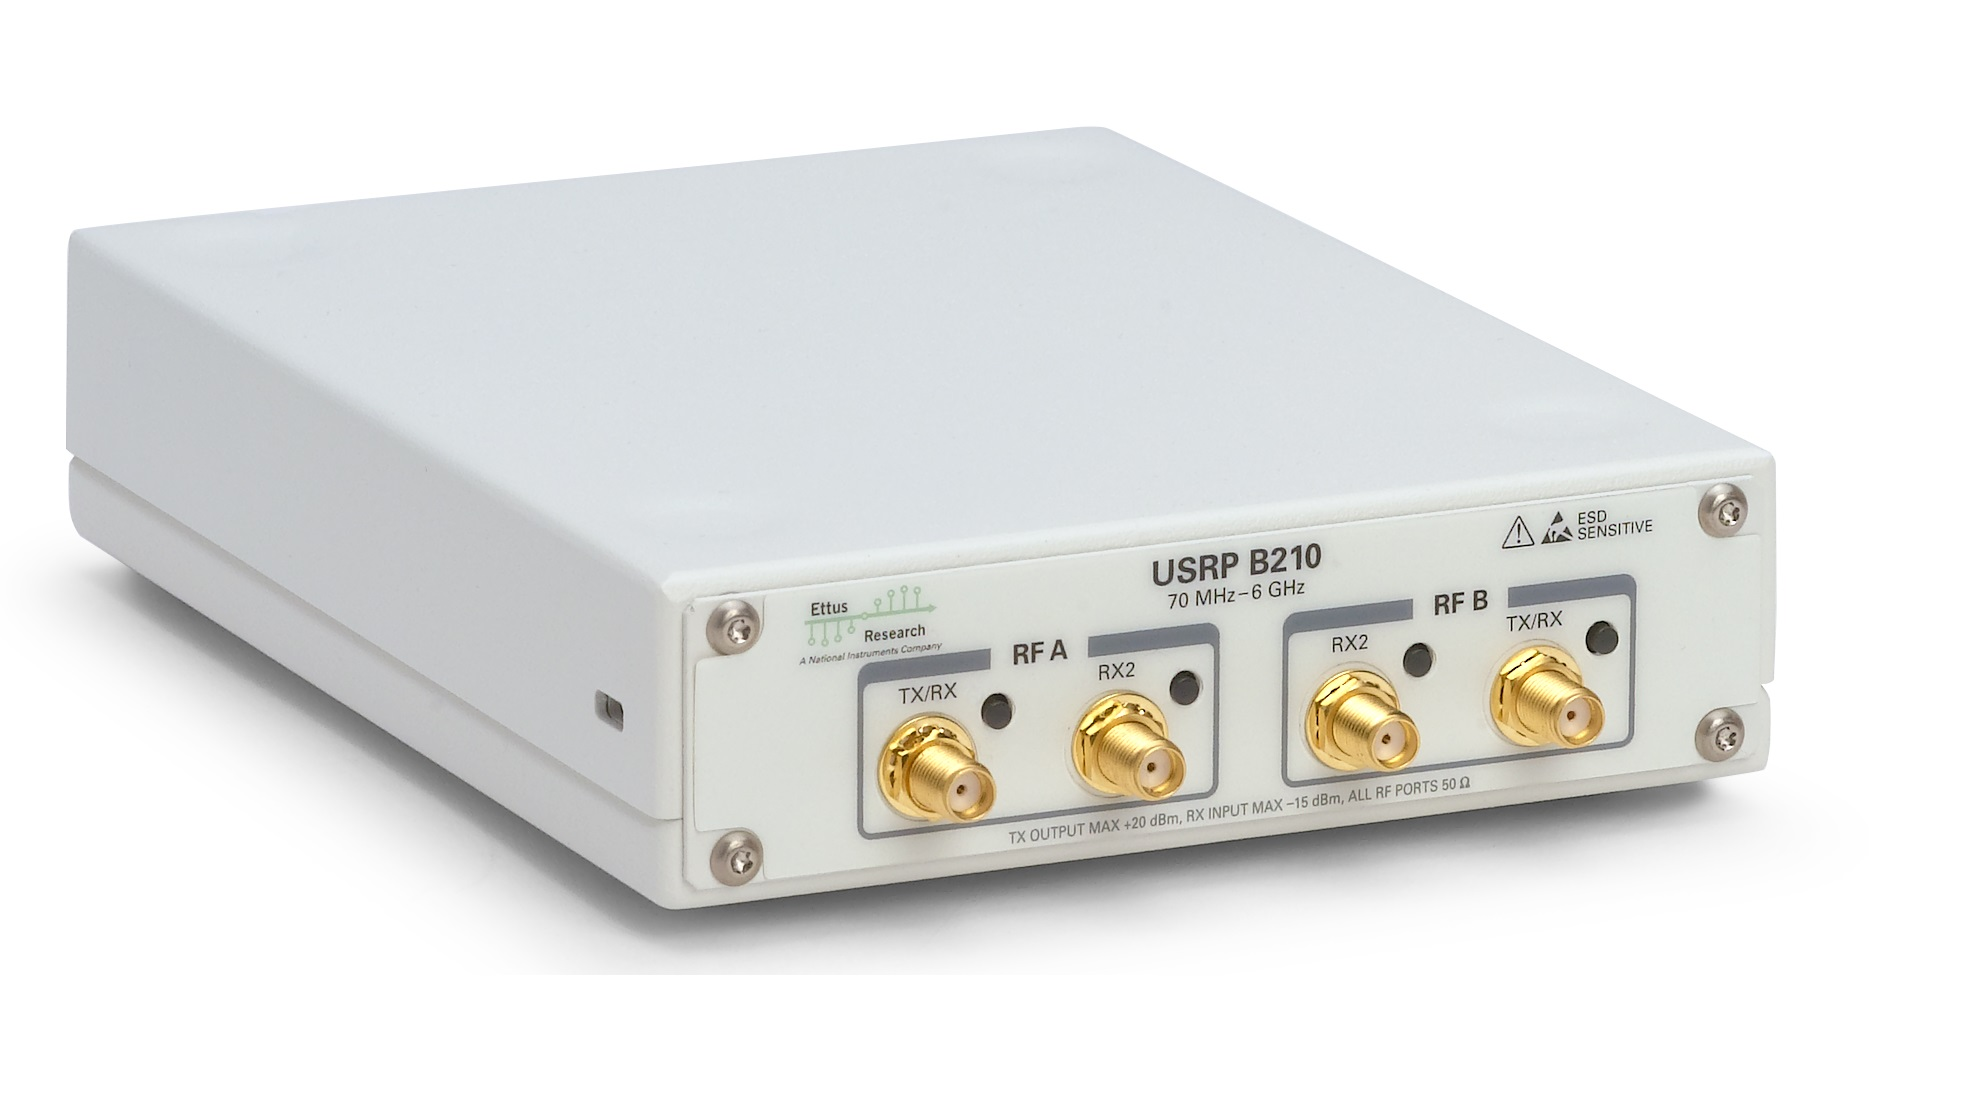
\includegraphics[width=\linewidth]{pics/bab2/B210.jpg}
			\caption{USRP B210 dengan \textit{enclosure}}
		\end{subfigure}
		\begin{subfigure}[b]{0.5\linewidth}
			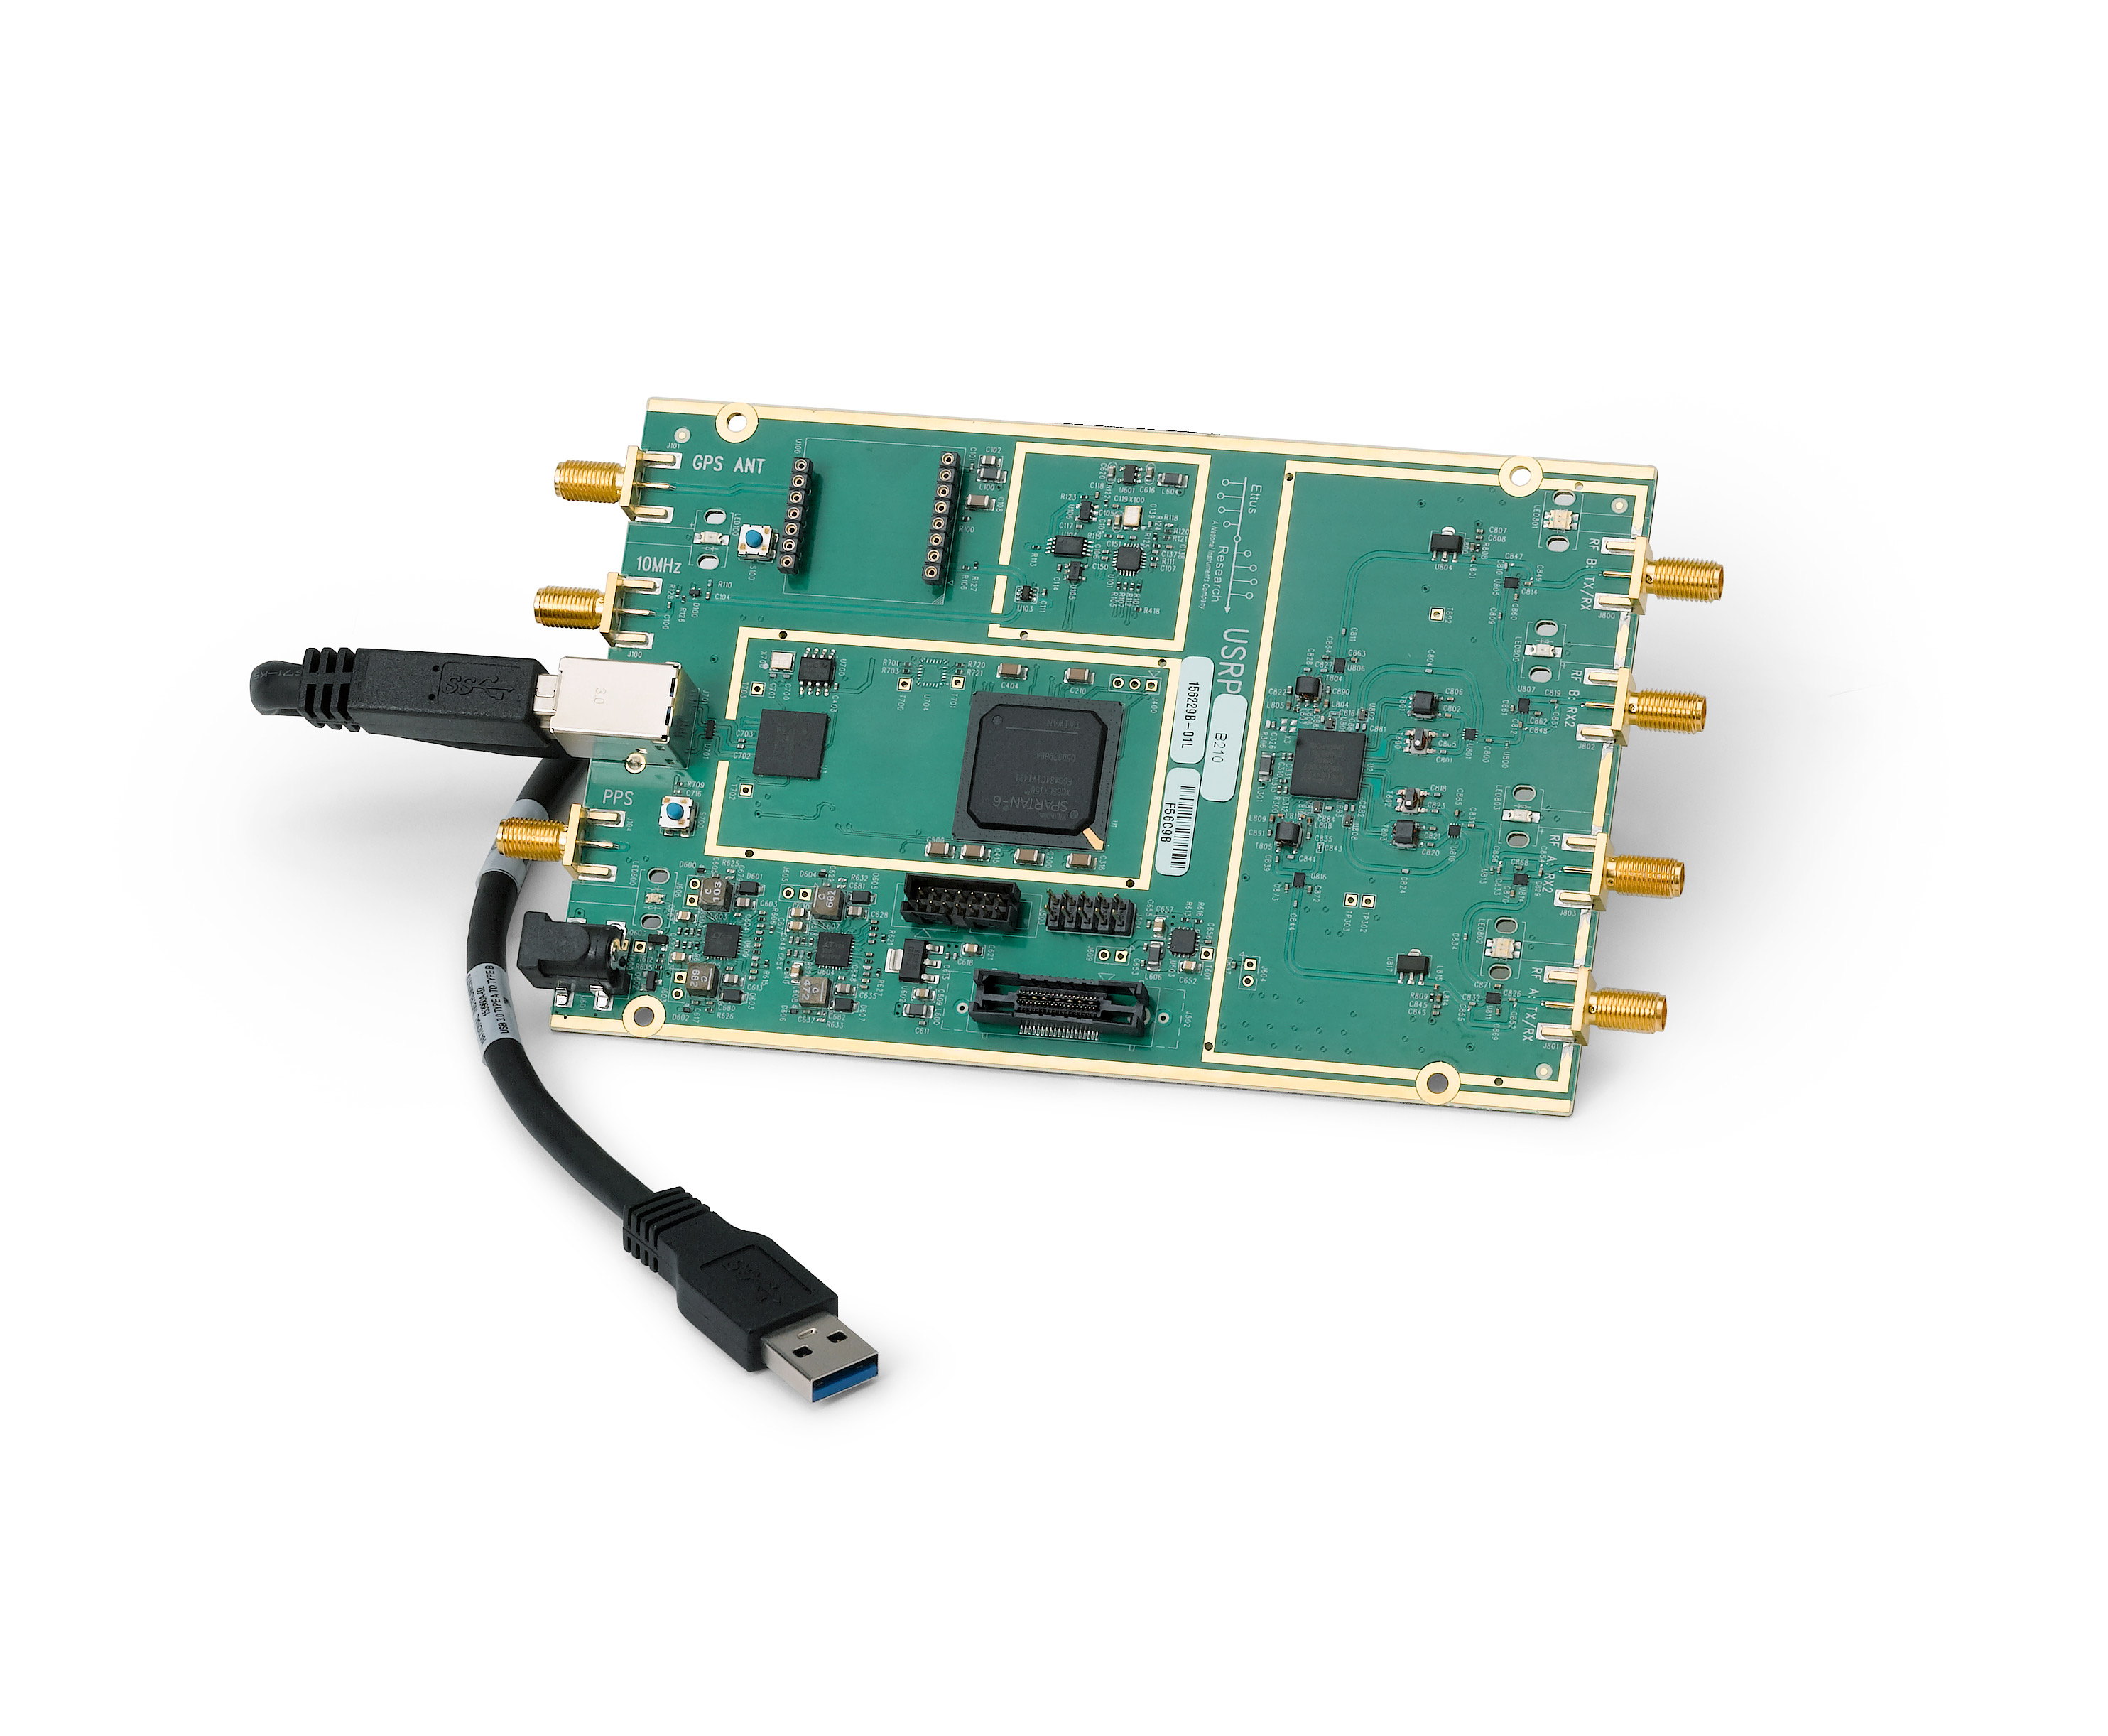
\includegraphics[width=7.3cm]{pics/bab2/B210Board.jpg}
			\caption{\textit{Board} USRP B210}
		\end{subfigure}
		\caption{USRP B210}
		\label{pic:gambarusrp}
	\end{figure}
\end{center}

\textit{Universal Software Radio Peripheral} atau yang sering disingkat dengan USRP merupakan \textit{platform} yang digunakan dalam mengimplementasikan SDR. Di dalam USRP terdapat \textit{Field Programmable Gate Array} atau FPGA(?) yang merupakan suatu \textit{Integrated Circuit} yang dapat diprogram. Pada hal ini, USRP adalah perangkat keras yang dapat menerima dan/atau mentransmisikan gelombang radio.

Kemampuannya untuk berinteraksi dengan gelombang radio inilah, ditambah pula dengan kemudahannya untuk melakukan pemrograman terhadap USRP ini yang membuat alat ini terkenal di kalangan akademisi dan peneliti. Karena pelaksanaan dan pengembangan prototipe menjadi lebih mudah dengan menghapuskan keperluan pengadaan komponen dalam prototipe.

Untuk melakukan antarmuka dan juga pelaksanaan pemrograman dengan USRP, dibutuhkan suatu perangkat lunak seperti \textit{Labview} dan GNURadio.

\subsection{\textit{GNURadio}}

\begin{figure}
	\begin{center}
		
\includegraphics[scale=0.5]{pics/bab2/GNU.png} 
		\caption[Logo GNURadio]{Logo GNURadio}
		\label{pic:logoGnuRadio}
	\end{center}
\end{figure}
GNURadio adalah aplikasi yang dapat melakukan pemrograman terhadap USRP lewat antarmuka. GNURadio merupakan \textit{software open source} sehingga semua orang dapat mengakses, mengubah, dan membagikan \textit{source code} dari program tersebut secara bebas. Dengan menggunakan aplikasi ini, perubahan parameter pada USRP dapat dilakukan dengan mudah.

%------------------------------
\section{Pengolahan Sinyal}

Dalam proses pengolahan sinyal, terdapat berbagai macam faktor yang perlu diperhatikan, khususnya pada proses pengolahan sinyal yang dilakukan oleh suatu radar. Hal ini diperlukan sehingga dapat melakukan pengambilan data yang selanjutnya akan dianalisis dengan baik. 

\subsection{Bentuk Sinyal} \label{BentukSinyal}
\begin{figure}
	\begin{center}
		\begin{subfigure}[b]{0.3\linewidth}
			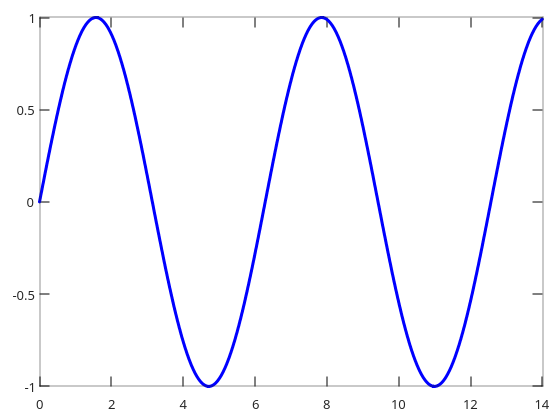
\includegraphics[width=\linewidth]{pics/bab2/gelsine.png}
			\caption[Gelombang Sinus]{Bentuk Gelombang Sinus}
		\end{subfigure}
		\begin{subfigure}[b]{0.3\linewidth}
			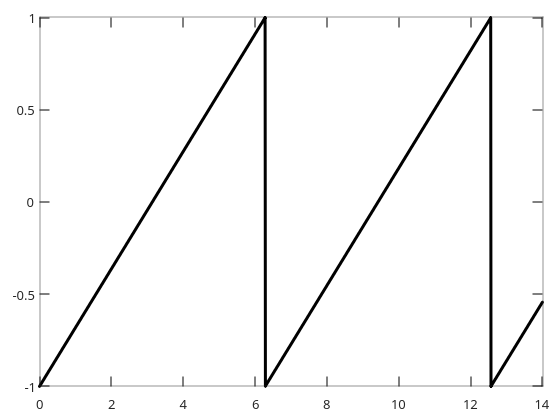
\includegraphics[width=\linewidth]{pics/bab2/gelsawtooth.png}
			\caption[Gelombang \textit{Sawtooth}]{Bentuk Gelombang \textit{Sawtooth}}
		\end{subfigure}
		\begin{subfigure}[b]{0.3\linewidth}
			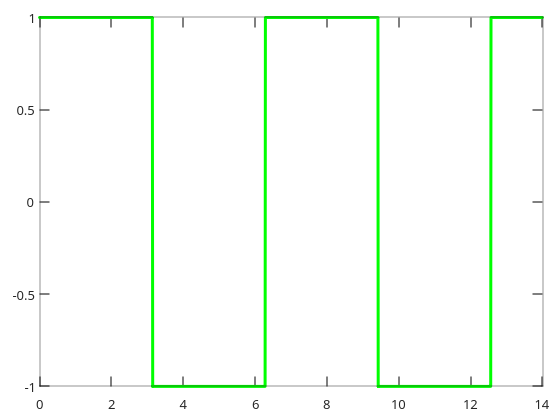
\includegraphics[width=\linewidth]{pics/bab2/gelsquare.png}
			\caption[Gelombang \textit{Square}]{Bentuk Gelombang \textit{Square}}
		\end{subfigure}
		\begin{subfigure}[b]{0.3\linewidth}
		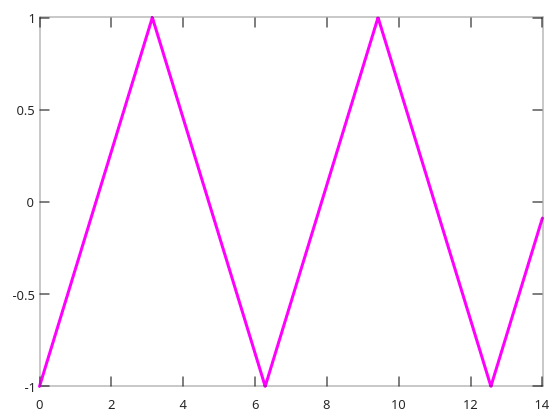
\includegraphics[width=\linewidth]{pics/bab2/geltriangular.png}
		\caption[Gelombang \textit{Triangular}]{Bentuk Gelombang \textit{Triangular}}
		\end{subfigure}
		\caption[Berbagai Bentuk Gelombang]{Berbagai Bentuk Gelombang}
		\label{pic:bentukGelombang}
	\end{center}
\end{figure}

Bentuk gelombang pada pengolahan sinyal merujuk pada saat suatu fungsi sinyal didefinisikan pada suatu waktu. Sinyal ini akan terus berulang secara periodik sesuai fungsinya masing masing. Berikut adalah persamaan dari tiap gelombang yang terdiri dari waktu ($t$), panjang gelombang ($\lambda$), amplitudo ($a$), dan fasa ($\phi$)

\begin{align}
	Sin &= a \sin \frac{2 \pi t - \phi}{\lambda} \\
	\textit{Sawtooth} &= \frac{2 a}{\pi} \arctan \tan \frac{2 \pi t - \phi}{\lambda} \\
	\textit{Triangular} &= \frac{2 a}{\pi} \arcsin \sin \frac{2 \pi t - \phi}{\lambda}
\end{align}

\subsection{Teknik Modulasi Frekuensi} 
Teknik modulasi merupakan salah satu teknik modulasi berdasarkan sudutnya, yang mana frekuensi dari gelombang \textit{carrier} akan termodulasi sesuai dengan gelombang masukan. Ilustrasi pada \ref{pic:modfrek} menunjukkan proses tersebut dengan baik. Ilustrasi pertama menunjukkan gelombang masukan, ilustrasi kedua menunjukkan gelombang \textit{carrier} yang akan dimodulasi, dan ilustrasi ketiga menunjukkan hasil gelombang yang telah termodulasi.
\begin{figure}
	\begin{center}
		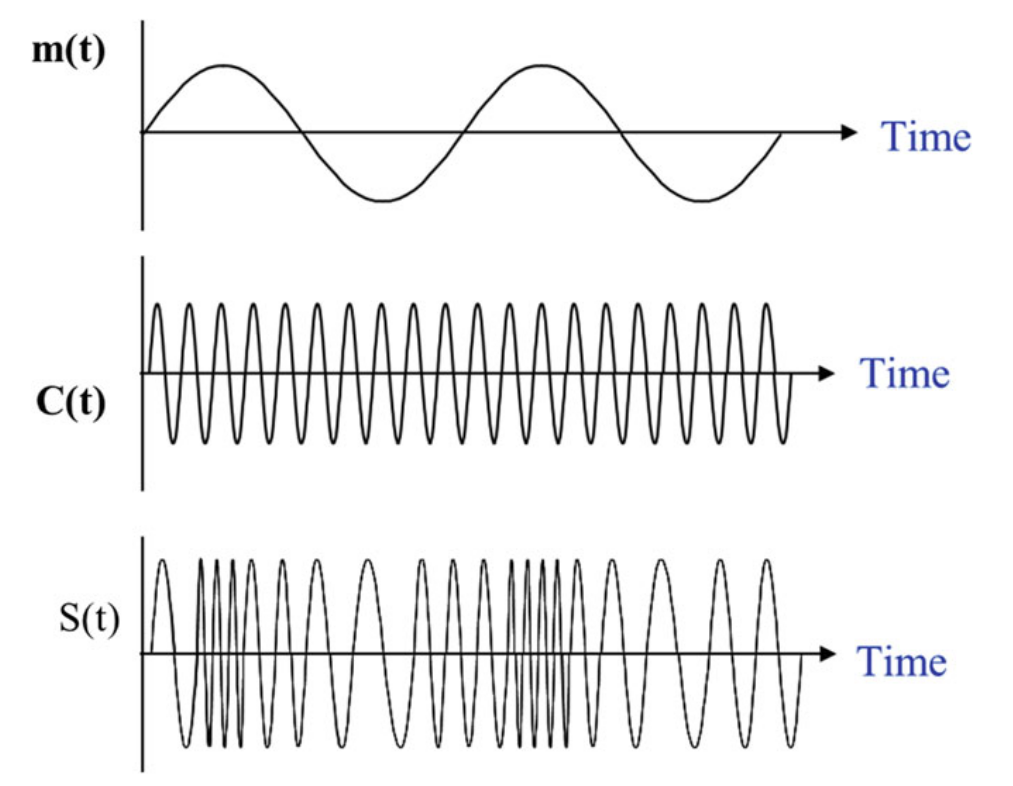
\includegraphics[scale=0.3]{pics/bab2/ilustrasimodfrek.png} 
		\caption[Modulasi Frekuensi]{Ilustraasi Modulasi Frekuensi \cite{Faruque2017}}
		\label{pic:modfrek}
	\end{center}
\end{figure}

\subsection{\textit{Frequency Modulated Continuous Wave}}
\textit{Frequency Modulated Continuous Wave} atau sering disingkat menjadi FMCW merupakan teknik transmisi gelombang elektromagnetik yang dilakukan secara kontinyu. Sesuai namanya, frekuensi dari sinyal yang ditransmisikan ini akan berubah terhadap waktu secara linear pada jangka \textit{bandwidth} tertentu \cite{Jankiraman2018}. Pada konteks penggunaan di radar, berbeda dengan teknik radar \textit{pulse} yang mengirimkan sinyal sekali dan menunggu sinyal yang tertransmisi untuk terpantul suatu objek dan kembali. 

\section{Radar}

Penggunaan gelombang elektromagnetik sebagai sarana untuk mendeteksi objek adalah konsep dasar dari radar. Radar sendiri merupakan singkatan dari \textit{Radio Detection and Ranging}, dari situ sangat nampak sekali tujuan dari penggunaan alat ini, yaitu untuk mendeteksi sesuatu dan mengukur jarak dengan menggunakan gelombang radio. 

Cara kerja dari radar adalah dengan memancarkan gelombang di dalam ruang bebas yang kemudian radar akan mendeteksi gelombang pantulan dari objek tersebut. Adanya gelombang yang terpantul ini tidak hanya menunjukkan keberadaan dari suatu objek, namun dengan membandingkan gelombang pantulan yang diterima dengan gelombang yang dikirimkan maka informasi tentang objek yang terdeteksi dapat didapat \cite{Skolnik2001}.

\subsection{Prinsip Kerja Radar}
\label{sect:prinsipKerjaRadar}
Pada gambar \ref{pic:skemaRadar} berikut, skema dan konsep dasar dari cara kerja radar dapat diamati. Terlihat bahwa sinyal yang dikirimkan akan mengenai target, dalam kasus ini adalah pesawat, lalu sinyal yang mengenai objek akan kembali dengan sinyal yang lebih kecil dengan amplitudo yang lebih rendah. Perubahan pada gelombang yang terpantul dapat menggambarkan perilaku yang sedang ditunjukkan oleh objek yang di deteksi, mulai dari pengurangan amplitudo hingga pergeseran fasa.

 \begin{figure}
	\begin{center}
		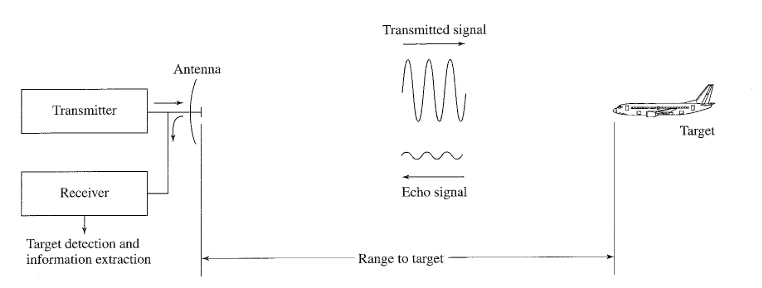
\includegraphics[scale=0.5]{pics/bab2/skemaradar.png} 
		\caption[Skema Dasar Radar]{{Skema Dasar Radar} \cite{Skolnik2001}}
		\label{pic:skemaRadar}
	\end{center}
\end{figure}

\subsection{Blok Diagram Radar}
 \begin{figure}
	\begin{center}
		\includegraphics[scale=0.4]{pics/bab2/blokdiagram.png} 
		\caption[Blok Diagram Radar]{{Blok Diagram Radar Sederhana \cite{Kingsley1999}}}
		\label{pic:blokdiagram}
	\end{center}
\end{figure}
Gambar \ref{pic:blokdiagram} menunjukkan blok diagram dari sistem radar pulsa sederhana. Dapat dilihat beberapa komponen yang membentuk seluruh sistem radar, semua komponen ini memiliki perannya sendiri sehingga proses pengiriman dan pendeteksian sinyal dapat dilakukan.  Bila seluruh sistem bekerja dengan baik, maka proses yang ditunjukkan pada penjelasan subbab \ref{sect:prinsipKerjaRadar} dapat berjalan dengan lancar.


\subsection{Persamaan Radar}
Persamaan radar berguna untuk menghubungkan seluruh komponen yang terdapat pada suatu sistem radar. Hubungan di antara seluruh komponen tersebut akan di perlihatkan secara matematis, sehingga penerapannya pada suatu alat akan terlihat dengan jelas. Dengan adanya beberapa persamaan ini, proses desain suatu radar akan menjadi lebih mudah dilakukan dan prediksi dari hasil radar yang dirancang bisa didapatkan.
\todo{Persamaan dari : \\
		Range to target\\
		Max. Unambiguous Range\\
		Power Density\\
		Power Density from directive antenna\
		Reradiated Power density back at radar\\
		Received signal\\ 
		Maximum range of radar\\
		Range Resolution}

\subsection{\textit{Radar Cross Section}}
\textit{Radar Cross Section} atau yang sering disingkat dengan RCS merupakan daerah suatu objek dari target yang dapat terdeteksi oleh suatu radar. Area tersebut diperhitungkan dengan mempertimbangkan bentuk dari objek dan interaksinya dengan gelombang elektromagnetik. Pada \ref{pic:RCS} ditunjukkan beberapa sifat RCS dan persamaannya.
\begin{center}
	\begin{figure}[h!]
		\begin{subfigure}[b]{0.5\linewidth}
			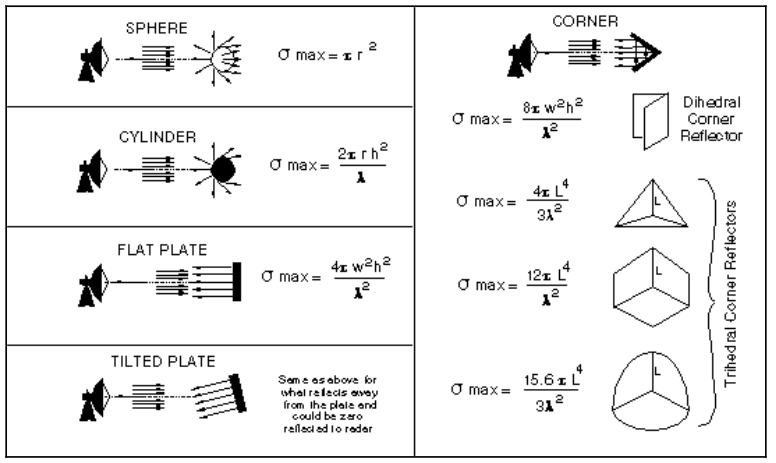
\includegraphics[width=\linewidth]{pics/bab2/rcsBentuk.png}
			\caption{Bentuk dan Persamaan \textit{Radar Cross Section}}
			\end{subfigure}
			\begin{subfigure}[b]{0.5\linewidth}
				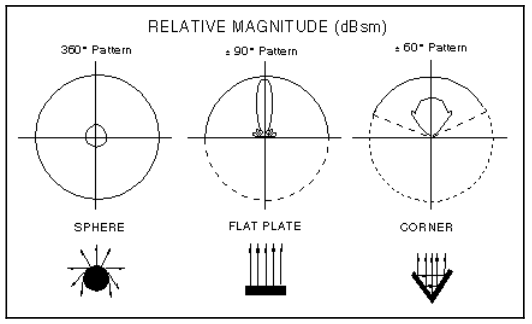
\includegraphics[width=\linewidth]{pics/bab2/rcsPola.png}
				\caption{Pola Radiasi dari \textit{Radar Cross Section}}
				\end{subfigure}
		\caption[\textit{Radar Cross Section}]{\textit{Radar Cross Section} \cite{ONeill2012}}
		\label{pic:RCS}
		\end{figure}
\end{center}

\subsection{Parameter Antena Radar}
Antena adalah bagian penting dalam sistem radar, karena antena berperan dalam memancarkan dan menerima gelombang elektromagnetik dari radar tersebut. Oleh karena itu berbagai spesifikasi dan parameter dari antena yang digunakan akan sangat berpengaruh terhadap radar yang akan dirancang.
\todo{Masukkan berbagai parameter antena yang berpengaruh dan ada di pers. radar}

\section{Pengolahan Sinyal Radar}

\todo{Tambah Kata Pengantar}

\subsection{Bentuk Gelombang Radar}
\begin{figure}
	\begin{center}
		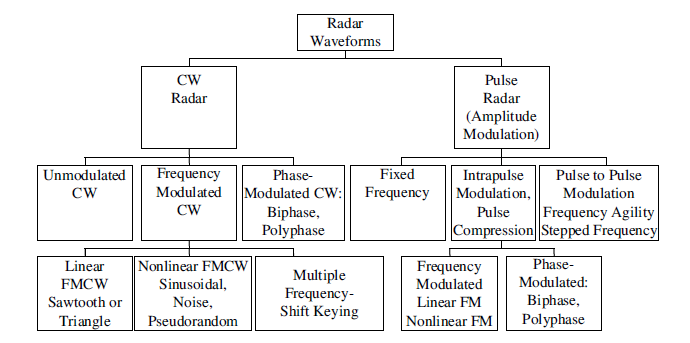
\includegraphics[scale=0.8]{pics/bab2/radarwaveform.png}
		\caption[Bentuk Gelombang Radar]{Bentuk Gelombang Radar \cite{Melvin2014}}
		\label{pic:bentukgelradar}
	\end{center}
\end{figure}
Bentuk gelombang radar dapat dibedakan menjadi dua kelas, yaitu radar dengan gelombang kontinyu dan radar pulsa. Seperti pada gambar \ref{pic:bentukgelradar}, kedua kelas tersebut masih dapat dibagi lagi kedalam beberapa teknik lain. Penggunaan salah satu jenis gelombang ditentukan berdasarkan kebutuhan radar yang akan di desain. 

Radar dengan gelombang pulsa akan memancarkan gelombang elektromagnetik dalam waktu singkat lalu jeda sejenak sesuai waktu yang ditentukan. Pada waktu jeda tersebut, radar akan mendeteksi sinyal pantul dari gelombang yang dikirim sebelumnya. Setelah waktu jeda berakhir, radar akan kembali memancarkan gelombang pulsa lagi. Radar dengan gelombang ini akan memancarkan gelombang elektromagnetik dengan \textit{power} yang tinggi. 

Sedangkan radar dengan gelombang kontinyu akan terus memancarkan serta menerima gelombang elektromagnetik tanpa henti dalam waktu yang bersamaan. Sehingga radar dengan gelombang kontinyu hanya digunakan pada sistem dengan \textit{power} yang rendah dengan jarak maksimum deteksi yang kecil. Hal ini disebabkan karena sering terjadinya kebocoran dari antena pengirim ke antena penerima. Alasan ini pula yang mendasari keputusan penggunaan \textit{power} yang rendah \cite{Scheer2015}.

\subsection{\textit{Frequency Modulated Continuous Wave Radar}}

Radar FMCW memancarkan sinyal yang bila terpantul objek, akan kembali terdeteksi. Kemudian sinyal yang diterima dicampurkan dengan sinyal yang dikirim, sehingga karena adanya \textit{delay} yang disebabkan oleh jarak gelombang bergerak, maka akan terdeteksi perbedaan frekuensi. Dengan begitu, perbedaan pada fasa dan frekuensi menjadi tolok ukur antara sinyal yang dikirim dengan sinyal yang di dapatkan kembali.
Oleh karena itu, salah satu karakteristik dari radar FMCW adalah bahwa jarak pengukuran dapat dihitung dengan membandingkan frekuensi sinyal yang diterima dengan sinyal yang ditransmisikan.   

\todo{Rumus Banyak}

\begin{align} 
	\Delta f_{FFT} &= \frac{1}{T}\\ 
	&= \frac{d(f)}{d(t) \cdot (f_{up} - f_{dwn})}
\end{align}
Keterangan = \\
\begin{tabular} {l c l}
	$\Delta f_{FFT}$ 						& = & Perbedaan frekuensi terkecil yang dapat diukur \\
	$\frac{d(f)}{d(t)}$ 					& = & Kecuraman terhadap frekuensi deviasi\\
	$f_{up}$ 									& =	& Batas atas frekuensi\\
	$f_{dwn}$								& = & Batas bawah frekuensi\\
\end{tabular}

\subsection{\textit{Linear Frequency Modulated Continuous Wave Radar}}
\textit{Linear Frequency Modulated}, yang juga sering disingkat sebagai LFM adalah teknik pengolahan sinyal yang dilakukan dengan menyapu frekuensi dari bawah ke atas (\textit{Up-Chirp}) atau dari atas ke bawah (\textit{Down-Chirp}). Dengan $f_{0}$ sebagai frekuensi tengah, dan dilakukan pada \textit{bandwidth} yang telah ditentukan. Teknik ini akan membantu pencapaian radar dengan resolusi yang lebih tinggi karena \textit{bandwidth} yang dicapai akan menjadi lebih tinggi.

Salah satu jenis gelombang LFM adalah \textit{Linear Triangular Frequency Modulation} yang ditunjukkan pada gambar \ref{pic:LFMTriangular}. Penggunaan jenis gelombang tersebut akan mempermudah proses evaluasi target.

\begin{figure}
	\begin{center}
		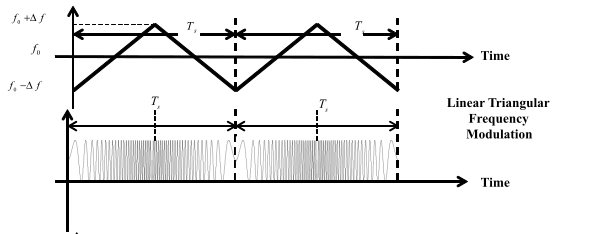
\includegraphics[scale=0.7]{pics/bab2/lfmTriangular.png}
		\caption[LFM Tipe Segitiga]{LFM Tipe Segitiga \cite{Jankiraman2018}}
		\label{pic:LFMTriangular}
	\end{center}
\end{figure}

\subsection{Stretch Processing}
Merupakan salah satu teknik \textit{Waveform Compression} yang digunakan untuk mendapatkan resolusi tinggi pada radar dengan meningkatkan \textit{bandwidth} dari sinyal. Salah satu teknik yang ada dalam kompresi gelombang adalah \textit{Stretch Processing} yang juga dijuluki dengan \textit{Active Correlation}. Teknik ini digunakan untuk memproses gelombang LFM dengan \textit{bandwidth} yang sangat besar.

\todo{Mengapa diperlukan\\ Terletak dimana? \\ Apa yang terjadi saat bekerja bersama LFM?}